%%%%%%%%%%%%%%%%%%%%%%%%%%%%%%%%%%%%%%%%%
% Beamer Presentation
% LaTeX Template
% Version 1.0 (10/11/12)
%%%%%%%%%%%%%%%%%%%%%%%%%%%%%%%%%%%%%%%%%

%----------------------------------------------------------------------------------------
%	PACKAGES AND THEMES
%----------------------------------------------------------------------------------------

\documentclass{beamer}

\mode<presentation> {

% The Beamer class comes with a number of default slide themes
% which change the colors and layouts of slides. Below this is a list
% of all the themes, uncomment each in turn to see what they look like.

%\usetheme{default}
%\usetheme{AnnArbor}
\usetheme{Antibes}
%\usetheme{Bergen}
%\usetheme{Berkeley}
%\usetheme{Berlin}
%\usetheme{Boadilla}
%\usetheme{CambridgeUS}
%\usetheme{Copenhagen}
%\usetheme{Darmstadt}
%\usetheme{Dresden}
%\usetheme{Frankfurt}
%\usetheme{Goettingen}
%\usetheme{Hannover}
%\usetheme{Ilmenau}
%\usetheme{JuanLesPins}
%\usetheme{Luebeck}
%\usetheme{Madrid}
%\usetheme{Malmoe}
%\usetheme{Marburg}
%\usetheme{Montpellier}
%\usetheme{PaloAlto}
%\usetheme{Pittsburgh}
%\usetheme{Rochester}
%\usetheme{Singapore}
%\usetheme{Szeged}
%\usetheme{Warsaw}

% As well as themes, the Beamer class has a number of color themes
% for any slide theme. Uncomment each of these in turn to see how it
% changes the colors of your current slide theme.

%\usecolortheme{albatross}
%\usecolortheme{beaver}
%\usecolortheme{beetle}
%\usecolortheme{crane}
%\usecolortheme{dolphin}
%\usecolortheme{dove}
%\usecolortheme{fly}
%\usecolortheme{lily}
%\usecolortheme{orchid}
%\usecolortheme{rose}
%\usecolortheme{seagull}
%\usecolortheme{seahorse}
%\usecolortheme{whale}
%\usecolortheme{wolverine}

%\setbeamertemplate{footline} % To remove the footer line in all slides uncomment this line
%\setbeamertemplate{footline}[page number] % To replace the footer line in all slides with a simple slide count uncomment this line

%\setbeamertemplate{navigation symbols}{} % To remove the navigation symbols from the bottom of all slides uncomment this line
}
%\usepackage{beamerthemeshadow}
\usepackage{graphicx} % Allows including images
%\usepackage{booktabs} % Allows the use of \toprule, \midrule and
\usepackage[brazil]{babel}
\usepackage[T1]{fontenc}
\usepackage[utf8]{inputenc}
\usepackage{amsthm,amsfonts,amssymb,amsxtra,empheq}
\usepackage{bm,amsmath,latexsym}
\usepackage{verbatim}
\usefonttheme[onlymath]{serif} % fonte modo matematico
%\renewcommand\mathfamilydefault{\rmdefault} % modo default modo matematico
\usepackage{animate}
\usepackage{filecontents}
	\begin{filecontents}{smallsizepause.txt}
		::0
		::1
		::1
		::1
		::2
		::3
		::4
		::5
		::6
		::7
		::8
		::9
		::10
		::11
		::12
		::13;
	\end{filecontents}

\theoremstyle{plain}
\newtheorem{exem}{Exemplo}
\newtheorem{teo}{Teorema}
\newtheorem{mot}{Motivação}
\newtheorem{defi}{Definição}
\newcommand{\iid}{\stackrel{\mathrm{iid}}{\sim}}
%----------------------------------------------------------------------------------------
%	TITLE PAGE
%----------------------------------------------------------------------------------------

\title[Variáveis Aleatórias Discretas: Distribuição Binomial, Distibuição Poisson e Distribuição Hipergeométrica]{Variáveis Aleatórias Discretas: Distribuição Binomial, Distibuição Poisson e Distribuição Hipergeométrica} % The short title appears at the bottom of every slide, the full title is only on the title page

\author{Ben D\^eivide} % Your name
\institute[UFLA] % Your institution as it will appear on the bottom of every slide, may be shorthand to save space
%{
%UFLA \\ % Your institution for the title page
%\medskip
%\textit{ben.deivide@gmail.com}\\ % Your email address
%\textit{www.benalana.blogspot.com}
%}
%\date{\today} % Date, can be changed to a custom date

\begin{document}

\begin{frame}
\titlepage % Print the title page as the first slide
\end{frame}

%\begin{frame}
%\frametitle{Sumário} % Table of contents slide, comment this block out to remove it
%\tableofcontents % Throughout your presentation, if you choose to use \section{} and \subsection{} commands, these will automatically be printed on this slide as an overview of your presentation
%\end{frame}

%----------------------------------------------------------------------------------------
%	PRESENTATION SLIDES
%----------------------------------------------------------------------------------------

%------------------------------------------------

\section{Revisão sobre variável aleatória}

  \begin{frame}
    \frametitle{Ilustração}
    \begin{center}
      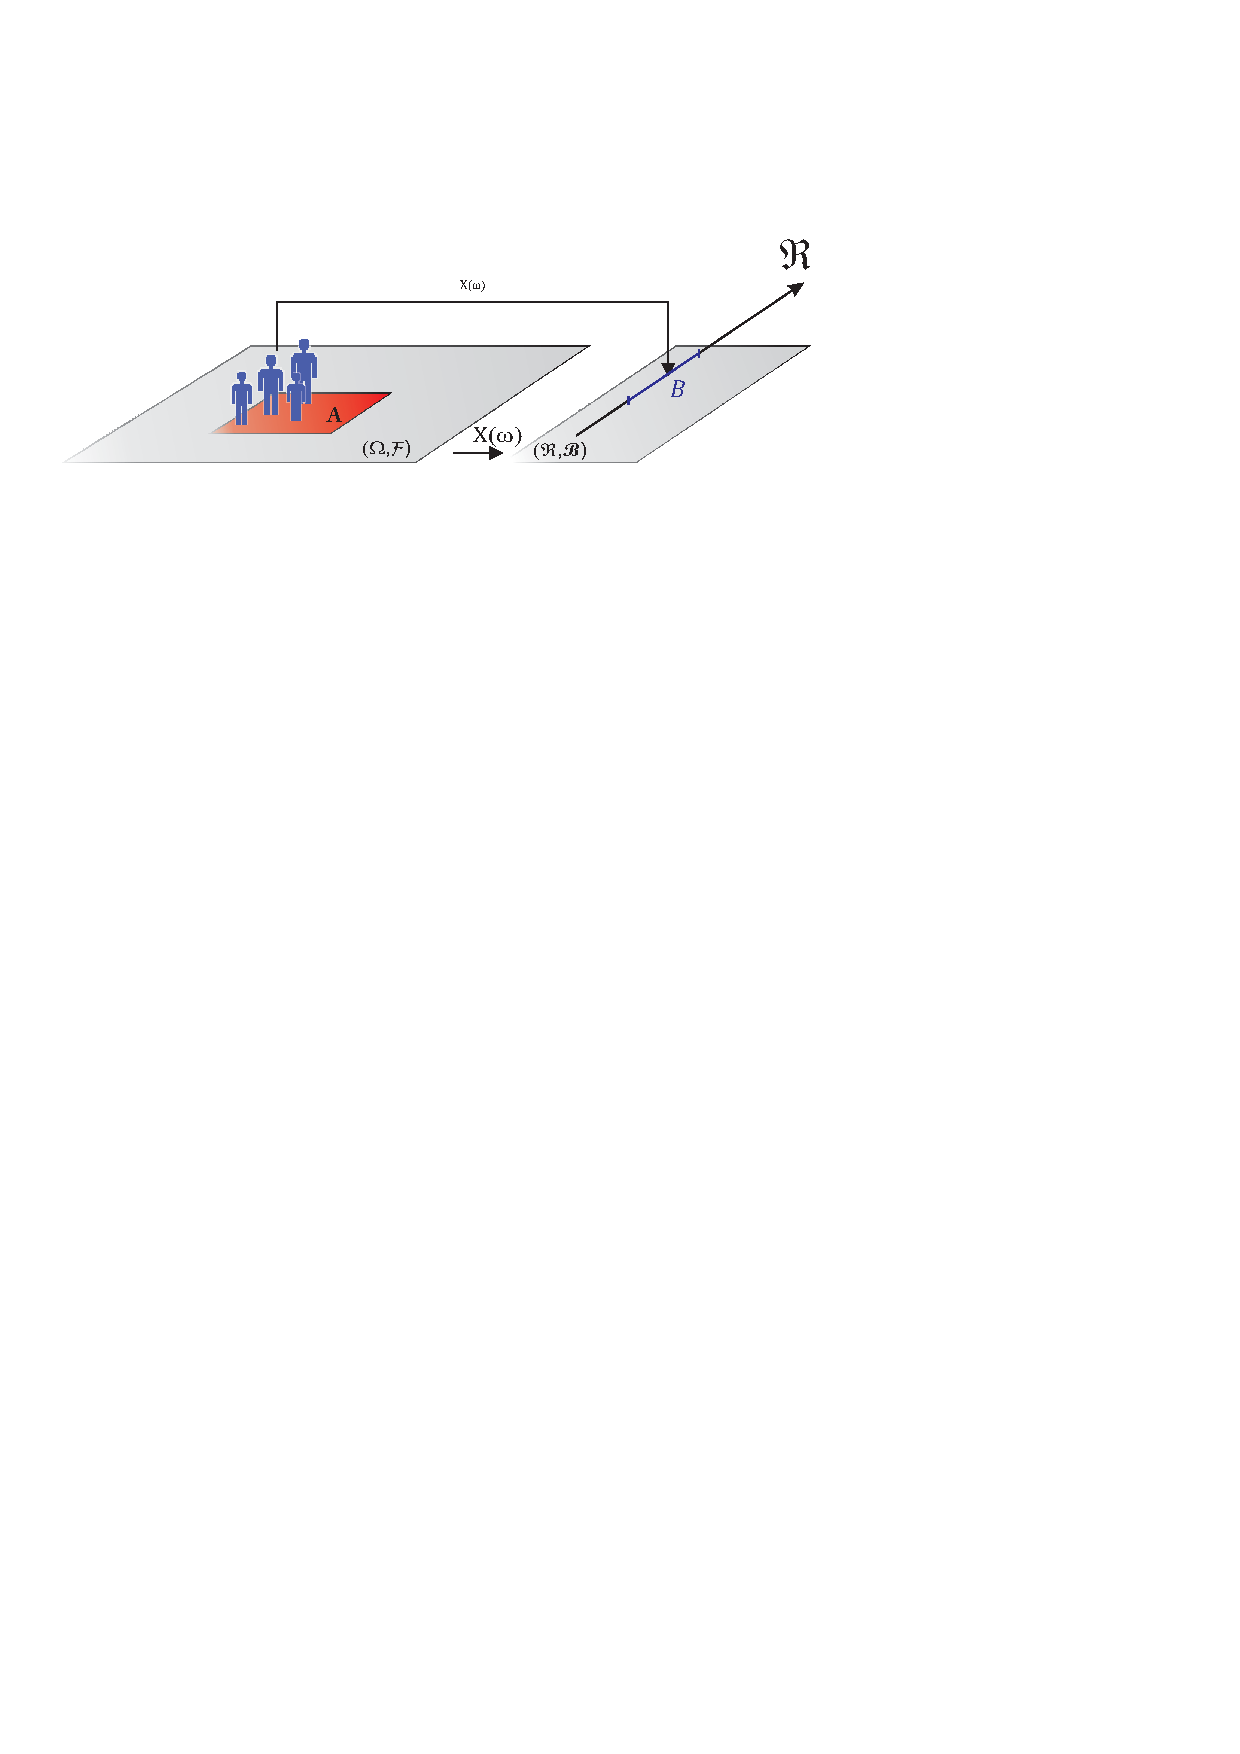
\includegraphics[scale = 0.9]{ranvar}
    \end{center}
  \end{frame}


\section{Variável aleatória discreta}


\begin{frame}
	\frametitle{Exemplos de Variável aleatória discreta}
	\begin{itemize}
		\item De todos os bits transmitidos através de um canal de transmissão digital, 10\% são recebidos com erro. Considere $X$ é uma variável aleatória discreta que representa o número de bits com erro nos próximos cinco bits transmitidos;\pause
		\item Uma máquina de produzir peças tem em sua produção 1\% de peças com defeitos. Considere $X$ é uma variável aleatória discreta que representa o número de peças com defeitos nas próximas 25 peças produzidas.
	\end{itemize}
\end{frame}

\begin{frame}
	\frametitle{Natureza da variável aleatória}
	\begin{defi}[Variável aleatória discreta]
		Uma variável aleatória $X$ discreta em $(\Omega, \mathcal{F}, P)$ é uma função que assume em uma sequência contável finita ou infinita $x_1,x_2,\ldots$ de números reais distintos, pertencentes a $B\in\mathcal{B}$, sendo $\mathcal{B}$ uma $\sigma$-álgebra de Borel.\qed
	\end{defi}
\end{frame}

\begin{frame}
	\frametitle{Caracterização da variável aleatória}
	\begin{defi}[Função de Probabilidade]
		Seja $X$ uma variável aleatória discreta, então sua função de probabilidade, $P_X:\mathbb{R}\rightarrow [0,1]$, é definida por:
		$$
		P_X(x)=P(X=x)=P(\{w\in\Omega:X(w)=x\}),
		$$
		sendo $\sum_xP_X(x)=1$.
	\end{defi}
\end{frame}


\begin{frame}
	%\frametitle{Caracterização da variável aleatória}
	\begin{defi}[Função de distribuição de uma v.a. discreta]
		A função de distribuição de uma variável aleatória discreta $X$ é a função $F_X:\mathbb{R}\rightarrow [0,1]$, definida por
		$$
		F_X(x)=P(X\leq x)=\sum_{\{i:x_i\leq x\}}P_X(X=x_i),
		$$
		para todo $x\in\mathbb{R}$.
	\end{defi}
\end{frame}


\begin{frame}
	\frametitle{Arremesso de uma moeda}
	Um experimento consiste em jogar uma moeda honesta três vezes e verificar a face superior, sendo $C$ o resultado cara e $K$ coroa.
	O espaço amostral para esse experimento é
	\begin{center}
		\animategraphics[controls, loop, width=0.9\textwidth]{2}{exem-moedas}{1}{20}
	\end{center}
\end{frame}

\begin{frame}
	\frametitle{Função de probabilidade e Função de distribuição}
	A função de probabilidade de $X$ é:
	\begin{align*}
	P(X = x) = \left\{
	\begin{array}{ll}
	1/8, & \textrm{para } x = 0,\\
	3/8, & \textrm{para } x = 1,\\
	3/8, & \textrm{para } x = 2,\\
	1/8, & \textrm{para } x = 3. 	
	\end{array}
	\right.
	\end{align*}
	A função de distribuição de $X$ é:
	\begin{align*}
	F(x) = \left\{
	\begin{array}{ll}
	0, & \textrm{para } x < 0,\\
	1/8, & \textrm{para } 0 \leq x < 1,\\
	4/8, & \textrm{para } 1 \leq x < 2,\\
	7/8, & \textrm{para } 2 \leq x < 3,\\
	1, & \textrm{para } x \geq 3. 	
	\end{array}
	\right.
	\end{align*}
\end{frame}

\begin{frame}
	\frametitle{Gráfico de FP e FDA}
	\begin{center}
		\animategraphics[controls, loop, width=0.9\textwidth]{2}{fpfdp}{1}{5}
	\end{center}
\end{frame}

\section{Distribuições especiais de variáveis aleatórias discretas}

  \begin{frame}
  	\frametitle{Distribuição Binomial}
  	\begin{center}
  		\animategraphics[controls, loop, width=0.9\textwidth]{2}{binom}{1}{18}
  	\end{center}
  \end{frame}

  \begin{frame}
  	\frametitle{Distribuição Binomial}
  	\begin{defi}[Distribuição Binomial]
  		Uma variável aleatória $X$ discreta, tem distribuição Binomial, se sua função de probabilidade é dada por
  		\begin{eqnarray}\label{eq:distbinomial}
  		P(X=x)=\left\lbrace \begin{array}{ll}
  		\binom{n}{x}p^x(1-p)^{n-x},& \textrm{ para } x= 0,1,2,\ldots,n,\\
  		0,& \textrm{caso contrário},
  		\end{array}\right.
  		\end{eqnarray}
  		em que $\binom{n}{x}=n!/[x!(n-x)!]$, e $p$ é o parâmetro do modelo \eqref{eq:distbinomial}, tal que $0 < p < 1$.
  	\end{defi}
  \end{frame}

  \begin{frame}
  	\frametitle{Exemplo da Distribuição Binomial}
  	\begin{exem}
  		\centering
      \animategraphics[controls, loop, width=0.7\textwidth]{0.5}{circint}{01}{08}
  	\end{exem}
  \end{frame}

  \begin{frame}
  	\frametitle{Exemplo da Distribuição Binomial}
  	\begin{exem}
  		Um produto eletrônico contém 40 circuitos integrados, que opera de modo independente. A probabilidade que algum circuito integrado tenha defeito é 0,01. O produto somente funcionará se não houver defeito em nenhum circuito integrado. Então, qual a probabilidade que o produto funcione corretamente?
  	\end{exem}
  \end{frame}

  \begin{frame}
  	\frametitle{Propriedades da Distribuição Binomial}
  	\begin{itemize}
  		\item Esperança:
  		\begin{align}
  		E[X] = np,
  		\end{align}
  		\item Variância:
  		\begin{equation}
  		Var[X]=np(1 - p).
  		\end{equation}
  		\item Desvio padrão:
  		\begin{equation}
  		\sigma_X = \sqrt{np(1 - p)}.
  		\end{equation}
  	\end{itemize}
  \end{frame}


  \begin{frame}
  	\frametitle{Distribuição Poisson}
  	\begin{center}
  		\animategraphics[controls, loop, width=0.9\textwidth]{2}{poisson}{1}{5}
  	\end{center}
  \end{frame}

  \begin{frame}
  	\frametitle{Distribuição Poisson}
  	\begin{defi}[Distribuição de Poisson]
  		Uma variável aleatória $X$ discreta, tem distribuição de Poisson, se sua função de probabilidade é dada por
  		\begin{eqnarray}\label{eq:poisson}
  		P(X=x)=\left\lbrace \begin{array}{ll}
  		\frac{e^{-\lambda}\lambda^{x}}{x!},& \textrm{ para } x= 0,1,2,\ldots,\\
  		0,& \textrm{caso contrário},
  		\end{array}\right.
  		\end{eqnarray}
  		em que o parâmetro $\lambda > 0$.\qed
  	\end{defi}
  \end{frame}

  \begin{frame}
    \begin{exem}
    	Os fios de cobre são muito utilizados em sistemas elétricos pela sua excelente condutividade elétrica, e apresentar uma resistência elétrica mais baixa entre todos os metais não-preciosos. Seja um experimento que observa as falhas de transmissão de um fio de cobre, e sabe-se que:
    	\begin{columns}
    		\begin{column}{5cm}
              \begin{center}
              	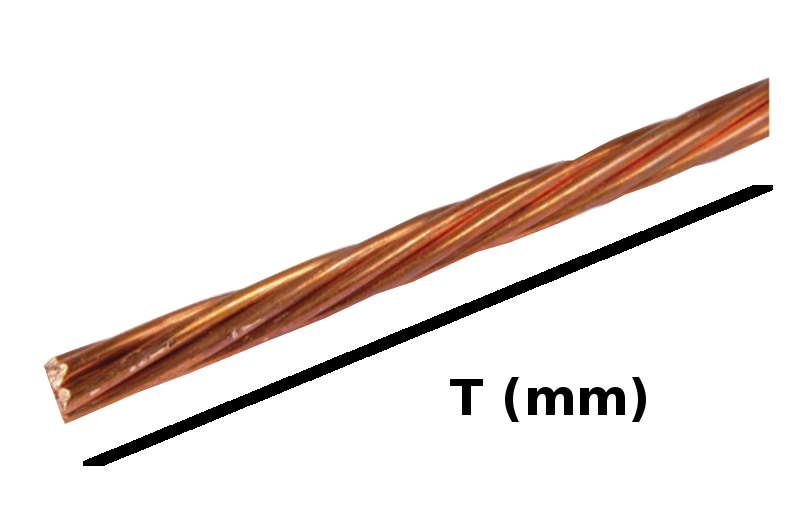
\includegraphics[scale = 0.6]{fiocobre}
              \end{center}
    		\end{column}
    		\begin{column}{5cm}
    		  \begin{itemize}
    		  	\item $\lambda$ = 2,3 falhas/mm;\pause
    		  	\item $X$ é uma variável aleatória que denota o número de falhas em cada 1 mm de cobre;\pause
    		  	\item P(X = 2 falhas/mm);\pause
    		  	\item P(X = 10 falhas/5mm).
    		  \end{itemize}
    		\end{column}
    	\end{columns}
    \end{exem}
  \end{frame}

  \begin{frame}
  	\frametitle{Distribuição Poisson}
  	As propriedades da distribuição Poisson:
  	\begin{itemize}
  		\item Esperança:
  		\begin{align}
  		E[X] & = \lambda,
  		\end{align}
  		\item Variância
  		\begin{equation}
  		Var[X] = \lambda,
  		\end{equation}
  		\item Desvio padrão
  		\begin{equation}
  		\sigma_X = \sqrt{\lambda}.
  		\end{equation}
  	\end{itemize}
  \end{frame}


  \begin{frame}
  	\frametitle{Distribuição Hipergeométrica}
  	\begin{center}
  		\animategraphics[controls, loop, width=0.9\textwidth]{2}{hipergeometrica}{1}{9}
  	\end{center}
  \end{frame}

  \begin{frame}
  	\frametitle{Distribuição Hipergeométrica}
  	  \begin{defi}[Distribuição hipergeométrica]
  	  	Uma variável aleatória $X$ discreta, tem distribuição hipergeométrica, se sua função de probabilidade é dada por
  	  	\begin{eqnarray}\label{eq:hipergeo}
  	  	P(X=x)=\left\lbrace \begin{array}{ll}
  	  	\frac{\binom{M}{x}\binom{N-M}{K-x}}{\binom{N}{K}},& \textrm{ para } \scalebox{0.7}{$\max\{ 0, N-M\} \leq x \leq \min\{K, M\}$}\\
  	  	0,& \textrm{caso contrário}, \label{eq:hg}
  	  	\end{array}\right.
  	  	\end{eqnarray}
  	  	em que $M \geq x$ e $N-M \geq K-x$.\qed
  	  \end{defi}
  \end{frame}

  \begin{frame}
  	\frametitle{Exemplo da Distribuição Hipergeométrica}
    \begin{exem}
    	\begin{center}
    		\animategraphics[controls, timeline=smallsizepause.txt, width=0.7\textwidth]{0.5}{megasena}{1}{14}
    	\end{center}
    \end{exem}
  \end{frame}

  \begin{frame}
  	\frametitle{Propriedades da Distribuição Hipergeométrica}
  	Propriedades da distribuição Hipergeométrica:
  	\begin{itemize}
  		\item Esperança:
  		\begin{align}
  		E[X] & = Kp,
  		\end{align}
  		\item Variância
  		\begin{equation}
  		Var[X] = Kp(1 - p) \frac{N - K}{N - 1},
  		\end{equation}
  		\item Desvio padrão
  		\begin{equation}
  		\sigma_X = \sqrt{Kp(1-p) \frac{N - K}{N - 1}},
  		\end{equation}
  		em que $p = \frac{M}{N}$ é a proporção de sucessos no conjunto de $N$ objetos.
  	\end{itemize}
  \end{frame}

\end{document} 